%\documentclass[runningheads]{llncs}
%
%%\usepackage[latin9]{inputenc}
%%\usepackage{amsmath,amsthm}
%%\usepackage{braket}
%%\usepackage{amsfonts}

% Used for displaying a sample figure. If possible, figure files should
% be included in EPS format.
%
% If you use the hyperref package, please uncomment the following line
% to display URLs in blue roman font according to Springer's eBook style:
% \renewcommand\UrlFont{\color{blue}\rmfamily}
%
%
%\begin{document}
%
%\title{Stochastic models for dynamical systems on graphs and applications to genetic activity}
\chapter{The model}\label{model}
\lhead[\fancyplain{}{\bfseries\thepage}]{\fancyplain{}{\bfseries\rightmark}}
Models of boolean networks proposed by Kauffmann are limited and can't represent perfectly biological networks because of some considerations: simple RBNs present cahotic behaviours and attractors are not sufficient to explain cellular differentiation.
In this Chapter we present the theoretical model of GRNs based on RBNs.

\section{The underlying philosophy of the model}
The dynamical model is a schematic representation of the activity of gene regulatory networks introduced in Chapter \ref{grn}. We have to discuss the assumptions the define the model from a biological 
point of view: the main criticism to a model is that its assumptions cannot be justified by the biological mechanisms. 
Our goal is to model the genetic activity related to a differentiation process of a cell: i.e. this activity is a stable long term activity whose stability
is probably controlled by biochemical mechanisms (i.e. methylation processes), but for cancer cells the control dynamics is not so efficient allowing
the evolution of different cell populations. Then we assume that this evolution is possible due to the competition of different genetic activities through
dynamical mechanisms that can be triggered by the external environmental signals.
In particular we assume:
\begin{itemize}
\item the long term genetic activity is determined by the presence of small genetic networks that have a stable active dynamical state;
\item there exists an eternal control mechanism: the subnetworks have control nodes that prevent the arise of the active state in the subnetwork if there
are set to the inactive state;
\item once the active state has been established in a subnetwork it remains stable in time without any stimulus, except if an inhibitory stimulus 
change the state of control nodes;
\item the stability and the controllability properties of a subnetwork depends from the existence of loops in the subnetwork: a loop may be related to the activation
of metabolic cycles in the cell that define the cell behavior;
\item each node of a subnetwork may represent the state of a gene that is connected and regulates the activation of other genes;
\item in the cell differentiation mechanism is defined by the competition of different subnetworks that interact in a inhibitory way;
%\item the mutation mechanism change the connectivity of the network: we may distinguish %between permanent changes and dynamical change (i.e. a connection
%may exist or non exist during time).
\end{itemize}
The complexity of the model is not a fundamental issue since we want to point out universal behaviors:  first of all the existence of bistability or bifurcation 
phenomena for simple model and the definition of control parameters.
%
\section{The mathematical model and related problems}
Here we studied the model dynamics in different situations using mathematical methods. The main idea is understand the dynamics of the models to point
out the universal properties that are robust and could explain the experimental data. The biological meaning of control parameters is a fundamental task
to apply the model to predict the results of new experiments.\par\noindent 
We consider a physical system that can be described by an weighted interaction network among nodes that can assume different
dynamical states (in the case of a gene network the states $\sigma\in \{0,1\}$ and we have models similar to spin models).
The interaction structure is defined by signed adjacency matrix $A_{ij}\in\{-1,0,1\}$ where the sign refers to a cooperative or antagonist interaction between the connected nodes. 
In the simplest case, we introduce a stochastic dynamics using the probability $p_i(\sigma, t)$ that the node $i$ is in the state 
$\sigma$ (we assume $\sigma>0$) at time $t$: in a deterministic approach $p_i(\sigma, t)=\delta(\sigma-\sigma(t))$
to denote that the node assume the state $\sigma=1$ with probability one. The evolution of a deterministic model
can be described by the equation
\begin{equation}
\sigma_i(t+1)=\Phi_i(\sigma(t))=\Theta\left (\sum_j A_{ij}\sigma_j(t)\right )
\label{evolnet}
\end{equation}
where $\Theta(x)\in[0,1]$ is a threshold sigmoidal function (we assume $A_{ii}=0$ to avoid self loops). \par\noindent
Remark: the dynamics is a information diffusion on the network. If we consider the linear system
$$
\zeta_i(t+1)=\sum_j A_{ij}\zeta_j(t)
$$
where $\zeta_i$ are non negative integers we have an equivalent dynamics since $\sigma_i=\Theta(\zeta_i)$ and it is possible
to study the linear system to derive some properties of the initial system. For example the relaxation time to the solution $\sigma_i=1$
$\forall\; i$ is for a given initial condition $\sigma^0_j=\delta_{jk}$ is $t=n$ such that the matrix $A^n$ has positive entries along the whole
$k$-th column. This mens that for each node $i$ there is a walk of length $n$ from the initial node $k$ to $i$.
\par\noindent
We also assume a cause-effect relation so that $A_{ij}$ is a directed
graph. The deterministic model is a Hopfield network (each node has at least an input and an output link; the environment nodes has only output links)
and one could study the equilibrium states and their stability. An equilibrium condition as follows is characterized as follows:
for each $i$ let
$$
Q_i(t)=\sum_j A_{ij}\sigma_j(t) 
$$
then $Q_i>0$ if $\sigma_i>0$ and vice versa.  Then $A_{ij}\ge 0$(i.e. $A_{ij}$ is a connectivity matrix for a directed network) 
implies that the non trivial equilibrium is $\sigma_i=1$: if $\sigma_k=0$ for some $k\in K$ then we have
$$
\sum_{j\notin K} A_{kj}\sigma_j=0
$$
so $A_{kj}=0$ for all $j\notin K$ and the network is disconnected. Then we have the trivial solution $\sigma_i=0$. For each equilibrium solution $\sigma^\ast$ we have a stability basin
$$
S_{\sigma^\ast}=\left \{\sigma \; | \; \lim_{t\to\infty} \sigma(t)=\sigma^\ast\right \}
$$
If $S_{\sigma^\ast}$ defined neighborhood of $\sigma^\ast$ the solution is stable or if $S_{\sigma^\ast}=\{\sigma^\ast\}$ the solution completely unstable. 
The stability of the origin depends on the existence of a Ljapounov function: let introduce the network activity
$$
\Sigma(t)=\sum_i \sigma_i(t)=\sum_i \Theta(Q_i(t-1))\ge \Sigma(t-1)
$$
since if each node has at least one input link, $A_{ij}=1$ implies $\sigma_j(t-1)\Rightarrow \sigma_i(t)=1$ and the activity cannot decrease. The solution $\sigma_i=0$
is completely unstable. If there would exists an equilibrium solution with $\sigma_k=0$ for some $k$ then we define $S_A$ the set of nodes s.t.
$$
i\in S_A\quad \Rightarrow \quad \sigma_i=0
$$
(obviously $\sigma_k\in S_A$). Let $S_{\bar A}$ the complement of $S_A$, the network dynamics implies
$$
0=\sum_j A_{ij}\sigma_j=\sum_{j\notin S_A} A_{ij}\sigma_j=0 \qquad \textrm{if}\quad i\in S_A
$$
so that $A_{ij}=0$ if $i\in S_A$ and $j\in S_{\bar A}$: i.e. there is not a cause-effect connection between $S_{\bar A}$ and $S_A$ and the state $\sigma_i=1$ for $i\in S_{\bar A}$
is an equilibrium state. Therefore we have as many equilibrium states as many partitions $S_A$ and $S_{\bar A}$ there exist such that $S_A$ triggers the activity of $S_{\bar A}$
but not vice versa. For any initial condition $\sigma_i(0)=\delta_{ik}$ the possible evolution are a periodic orbit or an equilibrium state: one can detect all the equilibrium conditions
by $\sigma^\ast$ by the condition
$$
\sigma_i^\ast=1\quad \textrm{if}\quad \sigma_i(t)=1\quad \textrm{for}\;\textrm{some}\quad t\ge 0
$$
The equilibrium states are a semigroup: let $\sigma^a$ and $\sigma^b$ two equilibrium states the
$$
\sigma^a\cup \sigma^b=\sigma^c
$$
is still an equilibrium. An example: if there exit a one directional loop $\gamma$ in the network and there is no output link
from $\gamma$ to the remaining nodes of the network then $\sigma_i=1$ for any $i\in \gamma$ is an equilibrium.
If the loop is simple (each node has a one input link and one output link) the equilibrium is neutral since any change
$\sigma_i=1\to\sigma_i=0$ creates a periodic orbit (the total activity is constant). But if we we add a link to the loop
then we get a stable solution since a single node can trigger the activity of two nodes and the equilibrium is an attractive
stationary state (see Figure \ref{fig:onecluster}). If a node is accidentally set to zero this anomaly propagates in the loop, 
until it reaches the node $4$ where it is annihilated by the activity of the node $(2)$. The average lifetime of a single perturbation
is the average path length to propagate to the node $(4)$ from the initial node (therefore it depends from the loop length or in case
of presence of many loops, the average path length is computed considering independent loops). 
\vskip .5 truecm 
\begin{figure}
\begin{center}
\begin{tikzpicture}
[->,>=stealth',shorten >=1pt,auto,node distance=3cm,
                    thick,main node/.style={circle,draw,font=\Large}]

  \node[main node] (1) {1};
  \node[main node] (2) [below left of=1] {2};
  \node[main node] (3) [below right of=2] {3};
  \node[main node] (4) [below right of=1] {4};

  \path[every node/.style={font=\small}]
    (1) edge node [left] {+1} (4)
    (2) edge node [right] {+1} (1)
        edge node {+1} (4)   
    (3) edge node [right] {+1} (2)
    (4) edge node [left] {+1} (3);
    \label{schema1}
\end{tikzpicture}
\end{center}
\caption{\emph{Example of random boolean network.}}
\label{fig:onecluster}
\end{figure}
\vskip .5 truecm
The boolean network models the propagation of information. By studying the stability problem of the solution $\sigma_i=1$ it is convenient to introduce the dual dynamics:
$$
\sigma_i^c(t+1)=\Theta\left (\prod_{j\sim i} A_{ij}\sigma^c_j(t)\right )=\prod_{j\sim i} A_{ij}\sigma^c_j(t)
$$
where $\sigma_i^c=1-\sigma_i$ is the dual state of the node and the product is restricted to the nodes connected to $i$
($A_{ij}\ne 0$): i.e. the node $(4)$ takes the state $\sigma^c=1$ only if both the nodes
$(1)$ and $(2)$ in that state at previous time. This dynamics is valid for any configuration of the network and the state $\sigma^c=1$
moves on the network until it reaches an absorbing state for which
$$
\prod_{j\sim i} \sigma^c_j(t)=0 \quad \forall \; i
$$
For a given stable equilibrium $\sigma^\gamma$ state associated to a loop $\gamma$ any environmental perturbation
that set to zero a activity of a node will destroy the equilibrium after a time equal to the number of the loop nodes minus one.
For example in the figure there are two loops $((1)\to (2)\to (3)\to (4))$ and $((2)\to(4)\to (3))$ if we set to zero the node 
$(4)$ after three iterations all the nodes will be in the zero state. The two loops are nit independent since one loops contains the other). On the contrary if we set to zero the node $(1)$ one loop remains active. This remark allows to introduce the concept of control node: a node is a control node if its state is able to 
force the state of the whole network. The effect of a thermal bath could be introduced by assuming that the state of a node
is defined as random variable that takes value $\sigma_i(t)=1$ with probability $p_i(t)$ where 
\begin{equation}
p_i(t+1)=\Theta_T\left (\sum_j A_{ij}\sigma_j(t)\right )
\label{stocdyn}
\end{equation}
and $\Theta_T(x)$ is a logistic function 
$$
\Theta_T(x)=\frac{1}{2}\left (1+\textrm{tgh}(x/T-\epsilon)\right )
$$
where $\epsilon$ measures to tendency of the network to be in the idle state when no stimulus is present.
The logistic function is a generic sigmoidal function we do not expect that the specific form of $\Theta_T(x)$ is critical for the results.
\par\noindent



Remark: since the values of $x$ are
quantized to integer in any case, if $\epsilon>T^{-1}$ the idle state is statistically attractive so $\epsilon$ could define a critical temperature
for the network activation. We recover the deterministic dynamics for $T\to 0$. As a stochastic process we have a Markov process (since
the realization of the variable $\sigma_i(t+1)$ depends only on the present state $\sigma_j(t)$ of the network \cite{K52}. The dynamics (\ref{stocdyn})
is a Markov field: the realization of the variable $\sigma_i$ depends only from the present state of the network (and not from past states) and
only from the states of the connected nodes $A_{ij}\ne 0$. The last condition (Markov field) means that the realizations of $\sigma_i(t)$
and $\sigma_j(t-1)$ are independent if the nodes are not connected. The transition probabilities depend from the state of the network
and one derives the average dynamics
\begin{equation}
<\sigma_i>(t+1)=p_i(t+1)=\left \langle \Theta_T\left (\sum_j A_{ij}\sigma_j(t)\right ) \right \rangle\simeq
 \Theta_T\left (\sum_j A_{ij}p_j(t)\right ) 
\label{avestoc}
\end{equation}
Then we have two possibilities: if the total average network activity tends to increase
\begin{equation}
\bar \Sigma(t+1)=\sum_i p_i(t+1) =\sum_i  \Theta_T\left (\sum_j A_{ij}p_j(t)\right ) > \bar \Sigma(t)
\label{condave}
\end{equation}
the equilibrium solution $\sigma_i=1$ is attractive, on the contrary we have a an average tendency to decrease the network activity. 
The situation is illustrated in the fig. \label{fig:crit}
\begin{figure}[h]
\label{fig:crit} 
\centering{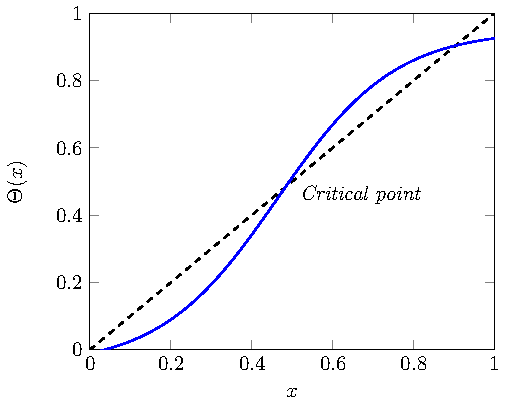
\includegraphics[scale=1.3]{images/theta.pdf}}
\caption{\emph{Possible behavior for the condition (\ref{condave}); the units are arbitrary and scale with the network dimension.}}
\end{figure}
Remark: the mean field approximation apply when the $\Theta_T(x)$ can be approximated by a linear function locally: i.e. the fluctuations are small
enough to approximate the function by a linear function in the whole fluctuation range. This is certainly not true when we have fat tail fluctuations.
\par\noindent
Except for a small initial region, the condition (\ref{condave}) can be satisfied up to a critical value of the network activity $\Sigma$ (if the temperature
is not too big), so that the average activity tends to increase. But if the activity is below the critical value then the network activity tend to decrease and
the stability of the solution $\sigma_i=1$ is lost. A connected network tends to be more stable since the quantities
$\sum_j A_{ij}\sigma_j$ increase.  This picture is clearly an approximation since we neglect the fluctuation effects: if the fluctuations are big (this
depends also on the connectivity matrix) we may have a fast transition between the two possible regime and a correction of the critical value. The
critical vale is a consequence of the sigmoidal behavior of the $\Theta_T(x)$ function and its depends on the temperature and on the $\epsilon$
values. In presence of fluctuations and of two dynamical regimes (active and non active) we expect that the network activity may switch from one regime
to another with a characteristic time scale (Kramer transition rate Theory, see Chapter \ref{kramer}). The transition may be triggered by large fluctuations that are both consequence
of rare events (in such a case the probability should be exponentially small with respect the activity) but also depend on the network structure (the presence of
hub nodes that can change the activity of many nodes amplifies the effect of small fluctuations (i.e. the change of the hub node state) and may introduce
fat tail statistic in the fluctuation distribution).
\par\noindent
Let us consider the existence of competitive networks (see Figure \ref{fig:comp}) that are linked by inhibitory links: if the first network is
in an exited state the second network should be completely switched off for a stable equilibrium.
\vskip .5 truecm

\begin{figure}
\centering
\begin{tikzpicture}[->,>=stealth',shorten >=1pt,auto,node distance=2.5cm,
                    thick,main node/.style={circle,draw,font=\Large}]

  \node[main node] (1) {1};
  \node[main node] (2) [below left of=1] {2};
  \node[main node] (3) [below right of=2] {3};
  \node[main node] (4) [below right of=1] {4};
  \node[main node] (5) [right of=4] {5}; 
  \node[main node] (6) [below right of=5] {6};
  \node[main node] (7) [above right of=6] {7};
  \node[main node] (8) [above left of=7] {8};

\path[every node/.style={font=\small}]
    (1) edge node [left] {+1} (4)
         edge[red] node [red] {-1} (8)
    (2) edge node [right] {+1} (1)
         edge node {+1} (4)   
    (3) edge node [right] {+1} (2)
    (4) edge node [left] {+1} (3)
    (8) edge node [left] {+1} (7)
    (5) edge node [right] {+1} (8) 
    (6) edge node [right] {+1} (5)
        edge[red] node [red] {-1} (3)
    (7) edge node [left] {+1} (6)
            edge node {+1} (5)  ;
\end{tikzpicture}
\caption{\emph{Example of a network composed by two competitive subnetworks.}}
\label{fig:comp}
\end{figure}
\par\noindent
If we start with all the node states set to one we create a frustrated situation, otherwise the network choose one
of the two possible stable states. In such a case the presence of an environmental noise could induce the transition
to one state to another (to be studied). An external forcing breaks the symmetry.\par\noindent
We expect a transition phase as a function of the temperature: increasing the temperature the node states tends 
to be independent, but under a threshold the system should choose a stationary state. 
\par\noindent
The system can be generalized to consider the interactions of different cooperative networks (possibly with different internal
structure) that are connected by inhibitory links (in the case of connection with excitatory links we join the subnetwork in a 
single one). We can introduce a metadynamics where $\nu_k(t)$ is the state of the $k$ subnetwork and
we have a relation
\begin{equation}
\nu_k(t+\Delta t)-\nu_k(t)=\phi(\nu_k(t))-\gamma\left (H_{kj}\nu_j(t)\right )
\label{metastoc}
\end{equation}
where $H_{hk}\ge 0$ is an inhibitory connectivity matrix. $\phi(\nu_k(t))$ describes the tendency of the sub-network to increase
its activity and $\gamma$ the average decreasing of the activity due to the presence of other sub-networks.
This is an effective equation: $\nu_k$ should describe the network activity (i.e. it could be the time-average activity of the nodes
assuming that the network could be considered in a stationary state). Indeed the evolution time scale $\Delta t$ could be assumed
$\Delta t\gg 1$ so that the subnetwork states are relaxed to a stationary states. 
The structure of attraction basins of the stable states could be related to a potential in the state space if
$$
\nu_k(t+1)-\nu_k(t)=-\frac{\partial }{\partial \nu_k}\left [ \frac{\gamma}{2} \sum_{ij}\nu_i H_{ij}\nu_j+\sum_j V(\nu_j)\right ]
$$
where 
$$
\phi(\nu)=-\frac{\partial V}{\partial \nu}
$$
Since $\phi(\nu)\ge 0$ $V(\nu)$ is increasing. Then we introduce the energy
$$
E=\frac{\gamma}{2} \sum_{ij}\nu_i H_{ij}\nu_j+\sum_j V(\nu_j)
$$
and the equilibrium are the critical points of the energy. Moreover 
\begin{eqnarray}
E(t+1)-E(t)&\simeq& (\nu_k(t+1)-\nu_k(t))\frac{\partial}{\partial \nu_k}\left [\frac{\gamma}{2} \sum_{ij}\nu_i(t) H_{ij}\nu_j(t)+\sum_j V(\nu_j(t))\right ]\nonumber \\
&=& -\frac{1}{2}\frac{\partial}{\partial \nu_k}\left [ \frac{\gamma}{2} \sum_{ij}\nu_i(t) H_{ij}\nu_j(t)+\sum_j V(\nu_j(t)) \right ]^2\nonumber
\end{eqnarray}
Therefore the energy is a Ljapounov function and the system equilibria are defined by the critical points of the Energy function
corresponding to local minima and maxima.\par\noindent
Remark: the existence of the Energy implies that $H_{ij}$ is symmetric negative defined
$$
\frac{\partial^2 E}{\partial \nu_j \partial \nu_i}=\frac{\partial^2 E}{\partial \nu_i \partial \nu_j}
$$
\par\noindent
The stochastic effect has to be introduce but it is possible a thermodynamics approach and a thermodynamics equilibrium exists
according to the Maxwell-Boltzmann distribution and the detailed balance condition. This means that the whole network does not
satisfy this condition, but the metadynamic network realized a reversible Markov process. The existence of a thermodynamic equilibrium
allows to use Maximal Entropy Principle and the Maxwell Boltzmann distribution when we introduce a thermal bath. 
\par\noindent
We are interested in networks with many different equilibria each one related to exited state of subnetworks (or a combination of subnetworks), 
in the effect of a thermal noise and in the effect of external forcing. The external  we introduce in the network boundary nodes whose state is defined by a given external signal
$\sigma_b(t)$ (possible a stochastic process) then the network dynamics reads
$$
\sigma_i(t+1)=\Theta\left (\sum_j A_{ij}\sigma_j(t)+\sum_b A_{ib}\sigma_b(t)\right )
$$
where $A_{ib}$ is the link between the environmental node $b$ and the node $i$. It is possible to introduce a probabilistic description of the evolution
of the probability that the network is in the state $\sigma'$ at time $t+1$ according to
\begin{equation}
p(\sigma',t+1)=\sum_{\sigma}\pi(\sigma',\sigma)p(\sigma,t)
\label{lapla}
\end{equation}
where
$$
\pi(\sigma'|\sigma)=E\left (\delta_{\sigma',\Phi_{\sigma_b}(\sigma)} \right )
$$
and the expectation value is computed on the realization of the input noise. $\pi(\sigma'|\sigma)$ is the transition rate per unit time (the continuous limit could be considered).
Let $\sigma_{eq}$ stable equilibrium state the effect of external random perturbations could be to move the network state in a neighborhood of the equilibrium solution
or it could induce a transition to other equilibrium basin attractions so that the dynamics starts to perform an intermittence behavior. In such a case the relevant quantities are  
the residence times in the different basins that can be associated to metastable states.
\par\noindent
We introduce the stochasticity in the system assuming that the adjacency matrix is not known: i.e. $A_{ij}$ is a extracted from an ensemble of random matrices.
As the result of an experimental one could assume that each entry $A_{ij}$ is a dichotomous random variable with probability $p_{ij}$ to get the value $\pm 1$ (i.e. the
link is active). The value $p_{ij}=0$ is admitted so that the corresponding link it always inactive. The problem is pointing out the existence of bifurcation phenomena so that it is possible to divide the ensemble in different communities with similar dynamical behaviors.
In the next Chapter we will focus on the implemantation of this model in order to do some analytical considerations and to analyse the dynamical process of networks made by two clusters.

\section{The model related to Kramer Theory}
Given a network made by two hinibitory clusters, the system will undergo bistable phenomena. As explained in Chapter \ref{kramer}, a bistable system can be represented by a stochastic process in which the stationary probability distributrion satisfies the Fokker Plank equation
\begin{equation}
\frac{\partial \rho}{\partial t } = \frac{\partial}{\partial x} V'(x)\rho + T \frac{\partial ^2 }{\partial x^2} \rho
\end{equation}

where we assume that the temperature $T$ is much les of the potential barrier $V_b - V_a$ and we look for a solution that reduces to the form:
$$
e^{-\frac{V(x)}{T}}
$$

We expect that the potential of the system should depend on the size of the clusters (the number of nodes of the clusters $N$) and on the average number of links in the clusters $K$:
$$
V = V(N,K)
$$
To estimate the potential we can measure the transition rates of the activity of the two clusters, using an ensemble of these networks. The probability distribution $\rho(\nu)$ can be constructed with the hisogram of the activities of the ensemble of double-clusters networks. 
